\documentclass{llncs}
%\pagestyle{headings} %page numbers
%\usepackage[font=small,labelfont=bf]{caption}


%% Language and font encodings
\usepackage[english]{babel}
\usepackage[utf8x]{inputenc}
\usepackage[T1]{fontenc}
\usepackage[outdir=./]{epstopdf}

\usepackage[]{xcolor}
%% Sets page size and margins
\usepackage[a4paper,top=3cm,bottom=2cm,left=3cm,right=3cm,marginparwidth=1.75cm]{geometry}

%% Useful packages
%\usepackage{amsmath}
\usepackage{graphicx}

\usepackage[colorinlistoftodos]{todonotes}
\title{Super awesome embeddings}
\author{Grzegorz Beringer \and Mateusz Jabłoński \and Piotr Januszewski \and Julian Szymański}
%

 \institute{
Faculty of Electronic Telecommunications and Informatics\\
Gda{\'n}sk University of Technology, Gda{\'n}sk, Poland
}

% (feature abused for this document to repeat the title also on left hand pages)

% the affiliations are given next; don't give your e-mail address
% unless you accept that it will be published
%\institute{Faculty of Electronics,
%Telecommunications and Informatics,
%Gdańsk University of Technology,
%ul. Narutowicza 11/12, 80-952 Gdańsk,
%Poland}

\begin{document}
\maketitle
\begin{abstract}
Abstract
\keywords{word sense disambiguation, word embeddings}

\end{abstract}

\section{Introduction}
\label{introduction}

\section{Related work}
\label{related work}

\section{Dataset}
\label{dataset}
For the purpose of testing word embeddings as a method to differentiate between different meanings, we gathered examples
for 6 ambiguous words, 4-7 meanings each (28 meanings in total). Ambiguous word together with its meaning constitues a
\textit{keyword}, which we use as a separate class when identyfing the closest meaning given some context. All keywords
can be seen on Figure 1.

\begin{figure}
    \label{fig:keywords}
    \caption{Ambiguous words with their meanings (keywords) from the dataset}
    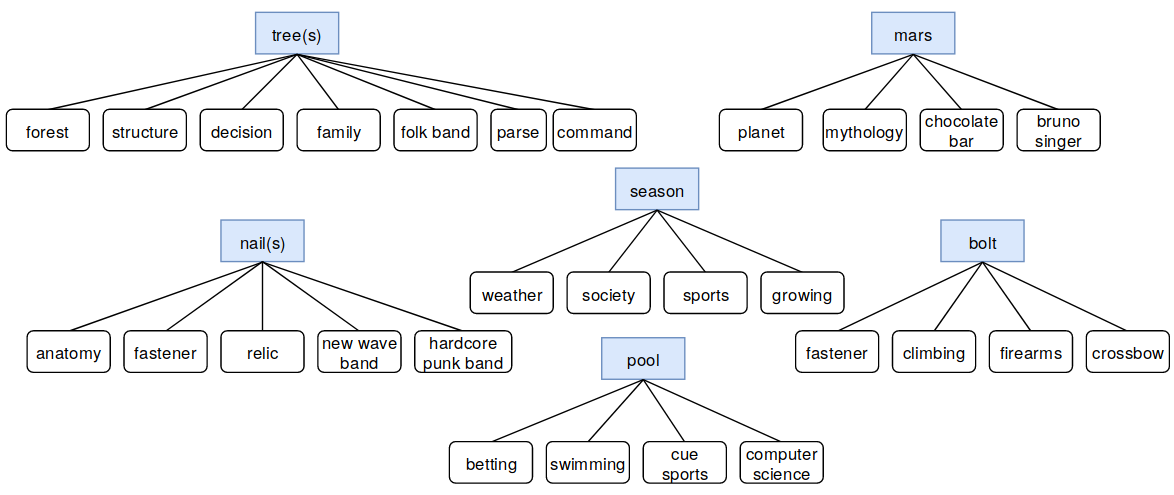
\includegraphics[scale=0.35]{res/keywords.png}
\end{figure}

Examples were mostly gathered from Wikipedia, using \textit{What links here} utility for each keyword. If usage examples
from Wikipedia were not enough, other websites were used (or even the Wiki article on specific keyword itself).

The dataset is split into training and test set, with 5 training and 10 test examples for each keyword. Each example
is stored in plain text, with the ambiguous word marked with "*" on both sides.

\bigskip
\underline{Example for \textit{bolt crossbow} keyword:}

\textit{"Sulfur- and oil-soaked materials were sometimes ignited and thrown at the enemy, or attached to spears, arrow and
*bolts* and fired by hand or machine. Some siege techniques—such as mining and boring—relied on combustibles and
fire to complete the collapse of walls and structures."}

\bigskip
The correct keyword for each example, together with a path to file and link, where the original text was taken from,
are stored in CSV files: \textit{train.csv} for training set, \textit{test.csv} for test set. Keywords themselves,
together with links to their Wiki articles, are stored in \textit{keywords.csv} file.

\bibliographystyle{splncs}
\bibliography{sample}

\end{document}


\begin{thebibliography}

\end{thebibliography}
